\section{Task Clarification}
Until now a model was developed and with this model settings for a PID controller were found. To test these settings on the real BalanBot, a Simulink model is needed, which implements the hardware specific functions. This includes reading the acceleration and gyroscope sensors, filtering them and writing to the output registers. This ensures that the BalanBot also moves in a different direction with a negative output of the controller than with a positive output. 

\section{Detailed Code Commentary}
\subsection{Sensor Data Reading}
The IMU communicates with the Arduino via the I2C bus. This must be implemented in the Simulink design. The sensor values obtained from this must now be further ground via Matlab function blocks. To get more trustworthy data in the later course of the program, a Kalman filter was also used. However, this filter needs both the measured angle and the measured yaw rate for proper operation. Therefore these two values were calculated. 

\begin{figure}[H]
    \centering
    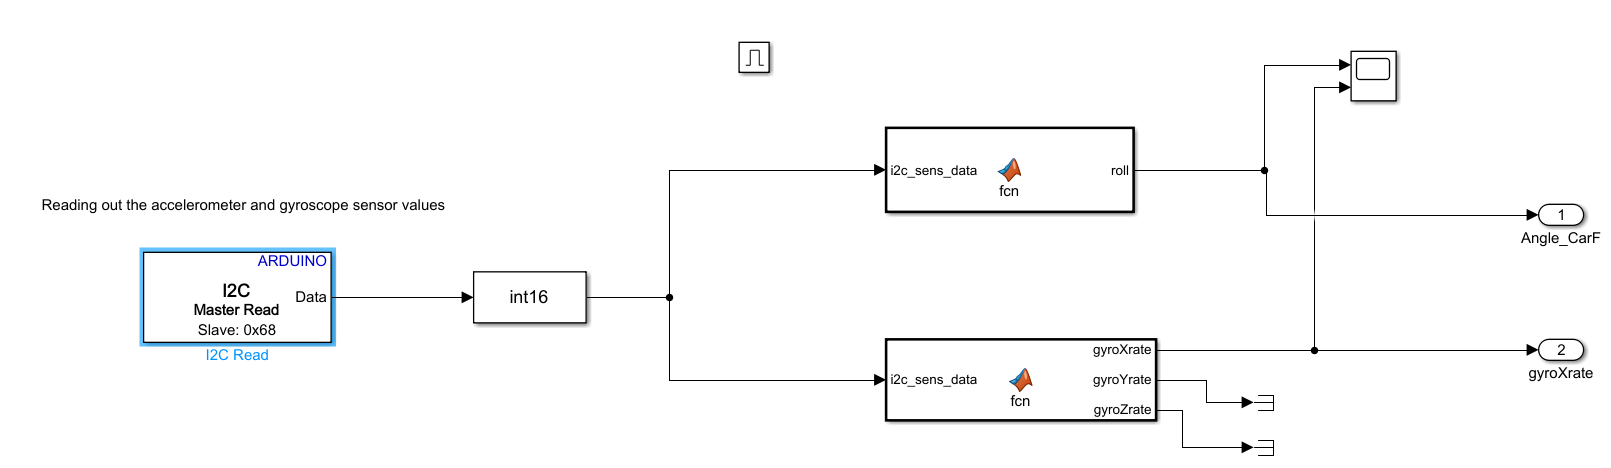
\includegraphics[width=\textwidth]{Lab_report/pics/hardware_impl/gyro_read.PNG}
    \caption{data reading Submodel}
    \label{fig:acc_gyro_read}
\end{figure}

\begin{lstlisting}[language=Matlab, caption=angle calculation]
function roll = fcn(i2c_sens_data)
    accX = double(i2c_sens_data(1));
    accY = double(i2c_sens_data(2));
    accZ = double(i2c_sens_data(3));
    roll = atan(accY / sqrt(accX * accX + accZ * accZ)) * 180/pi; 
end
\end{lstlisting}

\begin{lstlisting}[language=Matlab, caption=gyro rate calculation]
function [gyroXrate,gyroYrate,gyroZrate] = fcn(i2c_sens_data)
    gyroX = double(i2c_sens_data(5));
    gyroY = double(i2c_sens_data(6));
    gyroZ = double(i2c_sens_data(7));
    gyroXrate = gyroX/131;
    gyroYrate = gyroY/131;
    gyroZrate = gyroZ/131; 
end
\end{lstlisting}

\subsection{Data Processing}
In this submodel, the determined data is first filtered by means of a Kalman filter and then fed to the control algorithm. The data processing by means of this filter is described in more detail below.
\subsubsection{Kalman filter}
The principle of this filter is based on the estimation of the output quantity and the comparison of the measured output quantity. The difference of these two quantities is then weighted with the Kalman gain and used to correct the estimated output value. In our case the code for this estimation and correction algorithm is already finished and only a small test and proof of concept will be shown here. 


\subsubsection{Controller}

\subsection{Motor Control}